\documentclass[../master]{subfiles}

\begin{document}

\chapter{解析}
%\section{液体シンチレータの解析}
%\subsection{FADCの生データ}
%光電子増倍管から取得した波形データの一例を示す.
%
%\subsection{波形弁別 (n-$\gamma$ discrimination)}
%液体シンチレータのデータの中には中性子による信号とガンマ線による信号とが含まれている.
%この2つの波形には違いがあるので,その波形の違いから識別することができる.
%
%\subsection{中性子のレート}
%中性子線源から放出される中性子の量は時間とともに変化する.
%
\section{解析の概要}
MAIKo TCP の解析では背景事象の除去とトラック情報の抽出の2つが必要となる.
検出ガスには${}^{12}\mathrm{C}$だけでなく,陽子や${}^{4}\mathrm{He}$が含まれる.
そのため,中性子と陽子,${}^{4}\mathrm{He}$との散乱事象を取り除く必要がある.
中性子と${}^{12}\mathrm{C}$との散乱に対してトラックの情報を抽出する.
トラックの情報は中性子と${}^{12}\mathrm{C}$とが散乱した座標,
$\alpha$粒子が停止した点である.
anode image から$y, z$座標を,cathode image から$x, y$座標を決定することができる.
$x, z$座標は$\mu$-PIC のstrip 数に400 $\mu$mをかけることで決定できる.
$y$座標はTPC では荷電粒子が通過した位置から読み出し面に到達するまでの時間として測定される.
そのため,anode image, cathode image のclock にドリフトスピードをかけることで$y$座標を決定できる.
このようにして決定したanode image, cathode image の座標を合わせることで,
3次元の座標を決定することができる.

散乱点と停止点の座標から粒子が飛行した方向ベクトルと距離が決定される.
同じ粒子であれば,飛行距離から運動エネルギーが一意に決まる.
図\ref{fig::range_to_ene_alpha}に\Methane 50 hPa 中での荷電粒子の飛行距離と運動エネルギーの対応を示す.
飛行距離と運動エネルギーの相関はSRIM~\cite{srim}を用いて求めた.
\begin{figure}
  \centering
  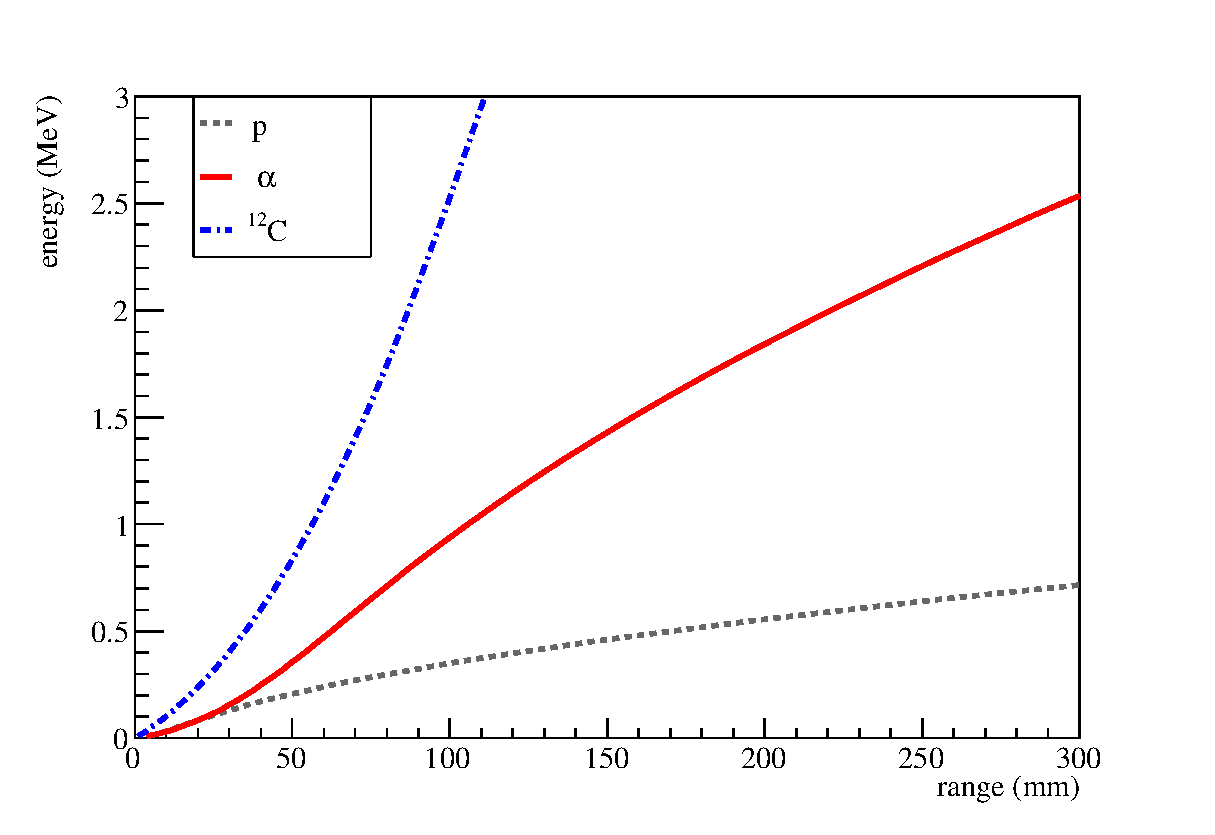
\includegraphics[clip, width=0.8\columnwidth]{range_to_ene.eps}
  \caption[\Methane 50 hPa 中での荷電粒子の飛行距離と運動エネルギー.]
          {\Methane 50 hPa 中での荷電粒子の飛行距離と運動エネルギー.
            この相関はSRIM を用いて求めた.
          }
  \label{fig::range_to_ene_alpha}
\end{figure}
この対応関係から粒子の運動エネルギーを決定する.
粒子の運動エネルギーを$T$,単位方向ベクトルを$(dx, dy, dz)$とすると,
4元運動量は
\begin{equation}
  p =
  \begin{pmatrix}
    E \\ p_{x} \\ p_{y} \\ p_{z}
  \end{pmatrix}
  =
  \begin{pmatrix}
    T + m \\ \sqrt{(T+m)^2 + m^2} dx \\ \sqrt{(T+m)^2 + m^2} dy \\ \sqrt{(T+m)^2 + m^2} dz
  \end{pmatrix}
  \label{eq::momentum_vector}
\end{equation}
となる.
決定した3つの$\alpha$粒子の4元運動量から${}^{12}\mathrm{C}$の4元運動量を再構成できる.
このようにして求めた4元運動量から${}^{12}\mathrm{C}$のエネルギー,散乱角度,励起エネルギーを求めることができる.

%\subsection{機械学習}
%これまではHough 変換を使って解析を行ってきたが,
%高速に処理をするためにニューラルネットワークを用いた解析方法を開発した.

\section{eye-scan}
本研究ではTPC の解析を人間の目 (eye-scan) で行った.
eye-scanでは,トラックの本数の識別と散乱点,停止点の抽出を行う.
ここではトラックの本数が3本であるイベントを${}^{12}\mathrm{C}(\mathrm{n},\mathrm{n}')3\alpha$イベントとした.
本研究では${}^{12}\mathrm{C}(\mathrm{n},\mathrm{n}')3\alpha$イベントに対して解析を行う.
検出ガスの決定のために,\ref{sec::triple_alpha_simulation}節のシミュレーションで生成したデータに対して解析を行った.

\subsection{検出効率}
${}^{12}\mathrm{C}(\mathrm{n},\mathrm{n}')3\alpha$イベントであっても,
各$\alpha$粒子のエネルギーや放出角度,トラックの太さによっては3つのトラックを区別することができない場合がある.
そこで,正しくトラックが3本と認識できる割合 (検出効率) を評価する.
評価は各ガスについて100 events ずつ行った.
検出効率を表\ref{tab::gas_summary}に示す.
%\begin{table}
%  \centering
%  \caption[シミュレーションデータに対する検出効率.]
%          {シミュレーションデータに対する検出効率.
%            検出効率は全イベントに対して3本のトラックをすべて認識できた割合である.}
%  \label{tab::detection_efficiency}
%  \begin{tabular}{cc}
%    \toprule
%    gas & 検出効率 (\%)\\
%    \midrule
%    \Methane & $55$ \\% \pm 7.42$ \\
%    \MethaneHydro & $91$ \\% \pm 9.54$ \\
%    \MethaneHerium & $78$ \\% \pm 8.83$ \\
%    \isoButaneHydro & $87$ \\% \pm 9.33$ \\
%    \isoButaneHerium & $90$ \\% \pm 9.49$ \\
%    \bottomrule
%  \end{tabular}
%\end{table}
\Methane 単体と\MethaneHerium 以外は約90\%の検出効率となっている.

%\subsection{検出効率の角度依存性}
\subsection{エネルギー分解能}
$\alpha$粒子の飛行距離の分解能により,エネルギー分解能が決まる.
そこで,eye-scanによる$\alpha$粒子のエネルギー分解能を評価する.
シミュレーションで粒子を生成した時に決定した$\alpha$粒子のエネルギー ($E_{\text{ideal}}$) と
eye-scanによって決定した$\alpha$粒子のエネルギー ($E_{\text{eye-scan}}$) の相関を
図\ref{fig::E_corr_ch4}, \ref{fig::E_corr_ch4_h2}, \ref{fig::E_corr_ch4_he},
\ref{fig::E_corr_ic4h10_h2}, \ref{fig::E_corr_ic4h10_he}に示す.
縦軸がシミュレーションで決定したエネルギー,横軸がeye-scanで決定したエネルギーである.
\begin{figure}
  \centering
  \begin{minipage}{0.45\columnwidth}
    \centering
    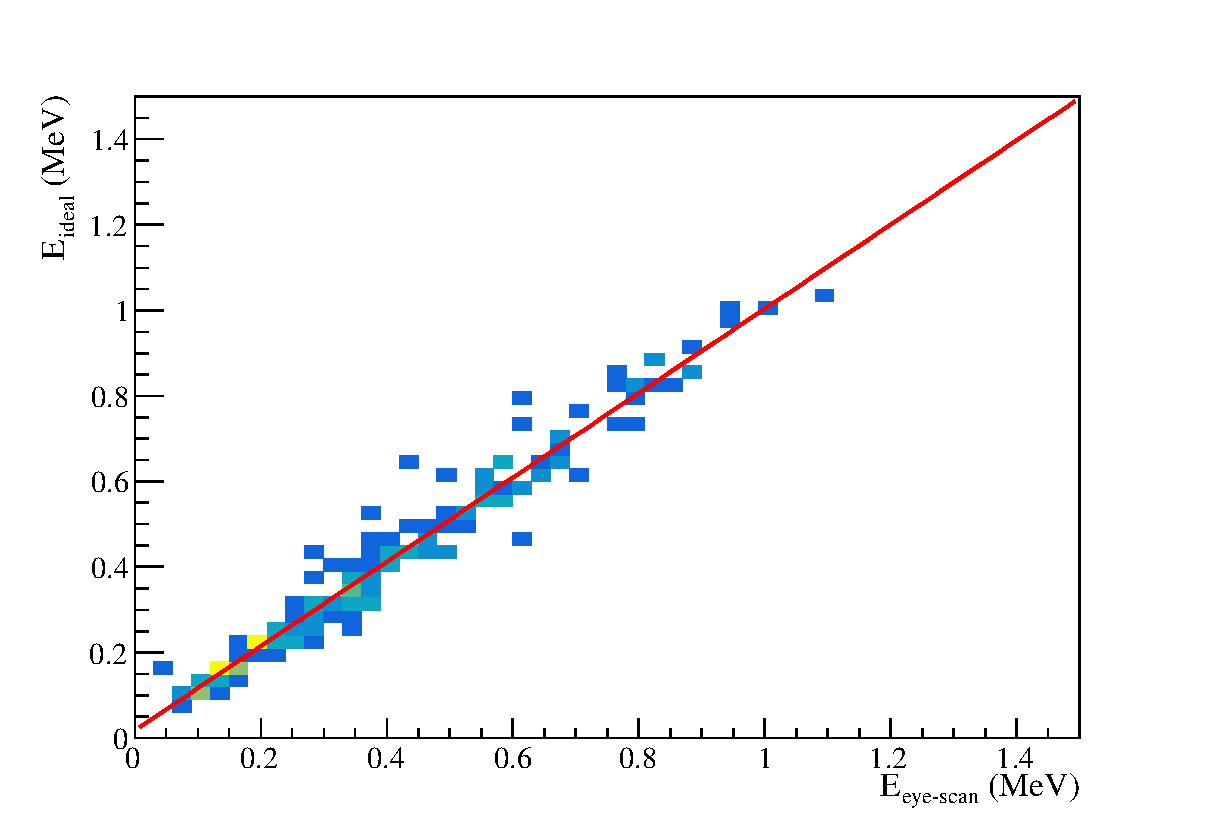
\includegraphics[clip, width=\columnwidth]{E_corr_10020.eps}
    \caption{\Methane の場合の$E_{\text{eye-scan}}$と$E_{\text{ideal}}$の相関.}
    \label{fig::E_corr_ch4}
  \end{minipage}  
\end{figure}
\begin{figure}
  \centering
  \begin{minipage}{0.45\columnwidth}
    \centering
    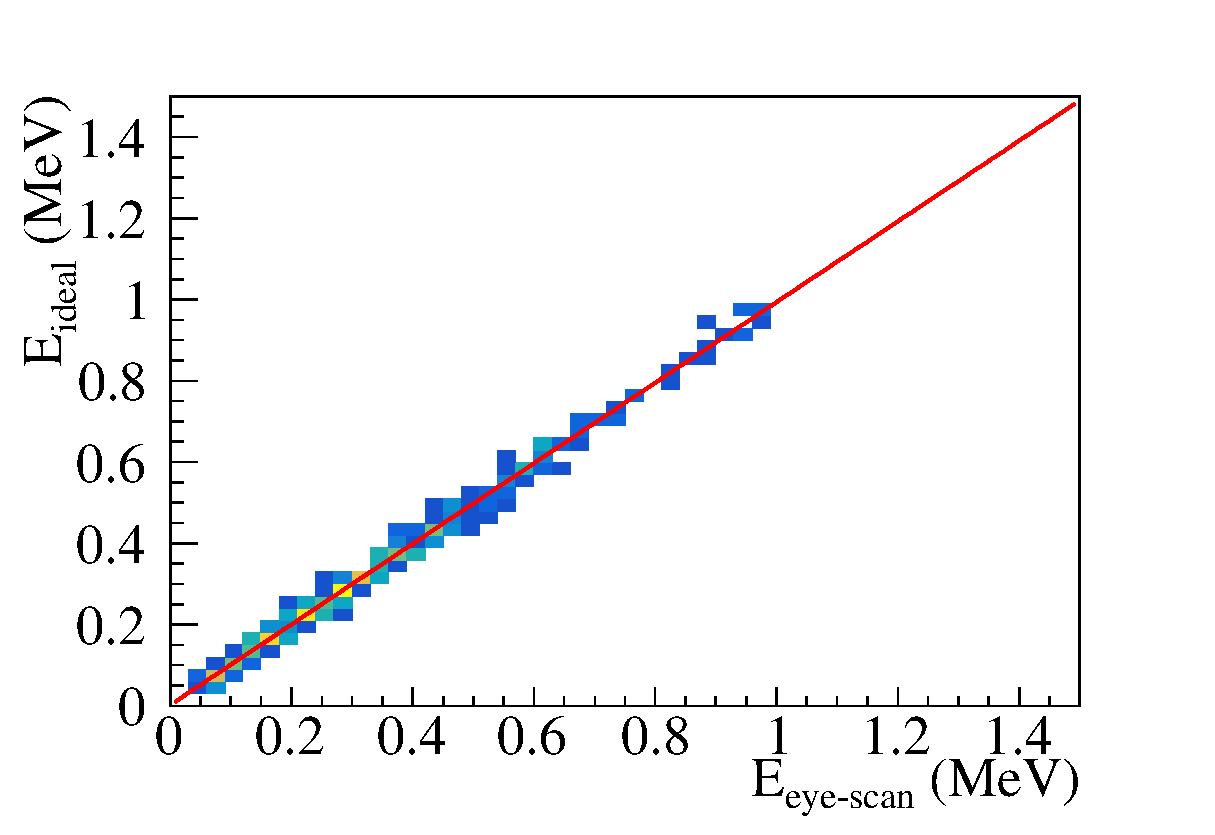
\includegraphics[clip, width=\columnwidth]{E_corr_10022.eps}
    \caption{\MethaneHydro の場合の$E_{\text{eye-scan}}$と$E_{\text{ideal}}$の相関.}
    \label{fig::E_corr_ch4_h2}
  \end{minipage}
  \begin{minipage}{0.45\columnwidth}
    \centering
    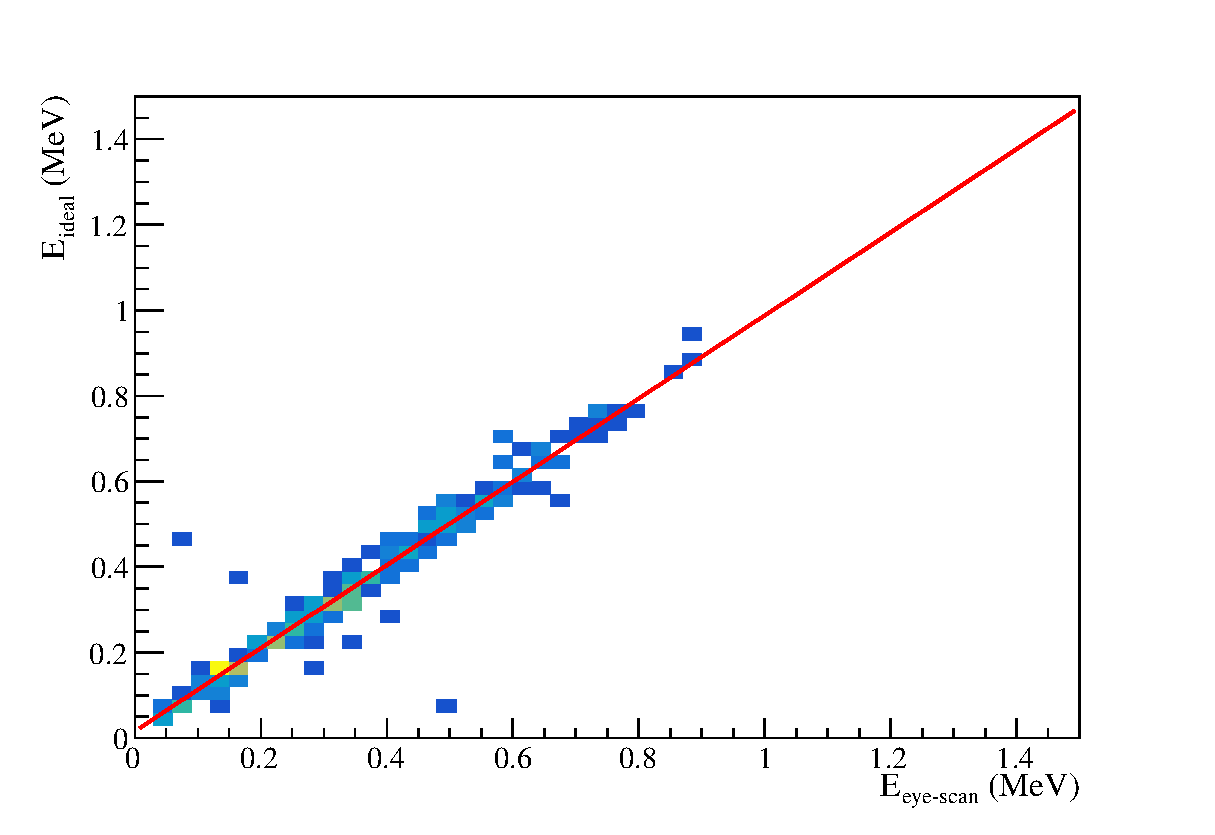
\includegraphics[clip, width=\columnwidth]{E_corr_10021.eps}
    \caption{\MethaneHerium の場合の$E_{\text{eye-scan}}$と$E_{\text{ideal}}$の相関.}
    \label{fig::E_corr_ch4_he}
  \end{minipage}
\end{figure}
\begin{figure}
  \centering
  \begin{minipage}{0.45\columnwidth}
    \centering
    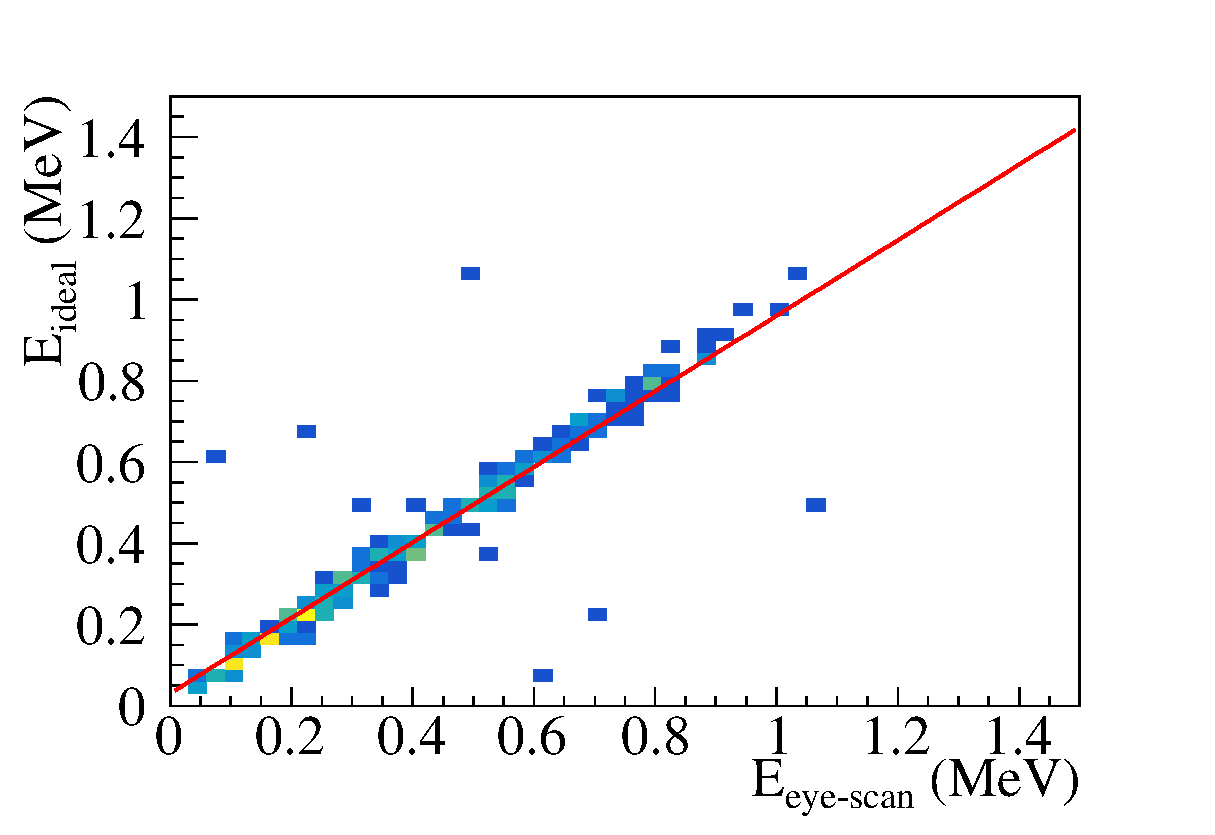
\includegraphics[clip, width=\columnwidth]{E_corr_10024.eps}
    \caption{iso-$\mathrm{C}_{4}\mathrm{H}_{1}\ (1) + \mathrm{H}_{2}\ (9)$の場合の$E_{\text{eye-scan}}$と$E_{\text{ideal}}$の相関.}
    \label{fig::E_corr_ic4h10_h2}
  \end{minipage}
  \begin{minipage}{0.45\columnwidth}
    \centering
    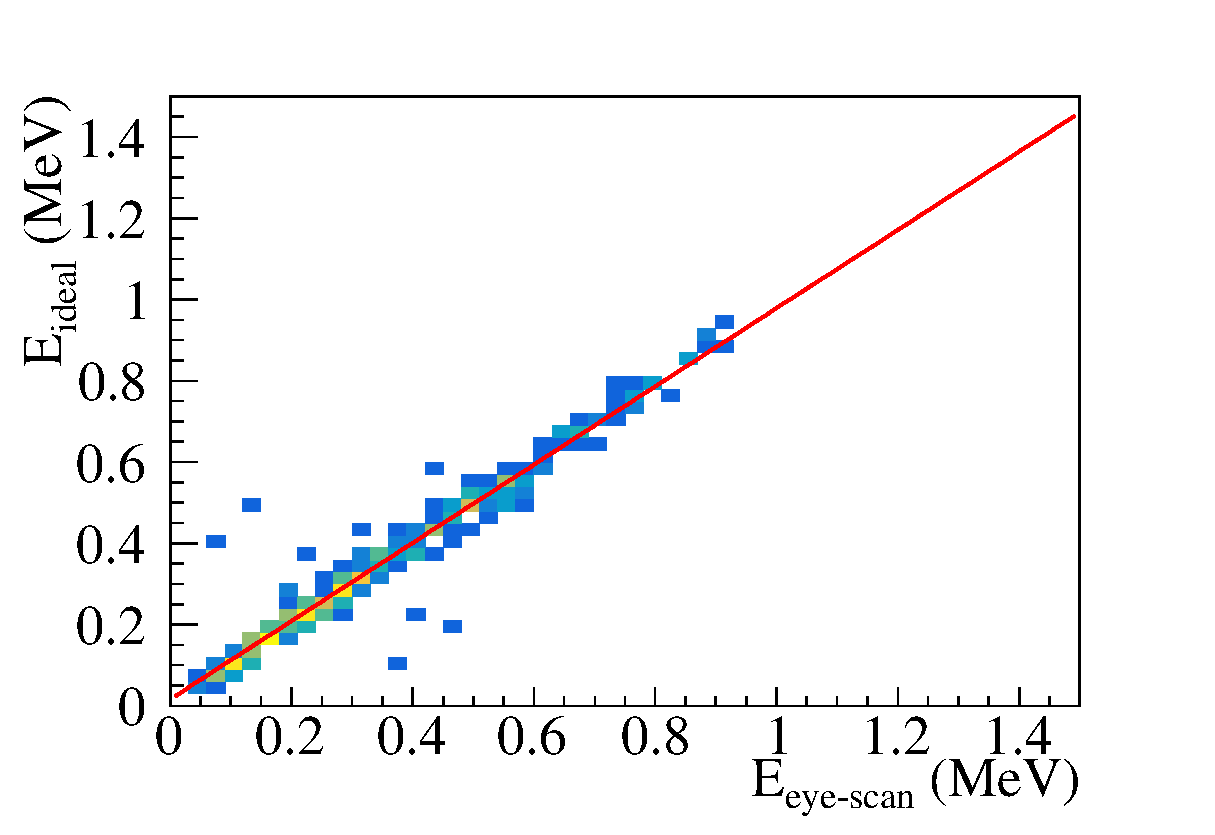
\includegraphics[clip, width=\columnwidth]{E_corr_10023.eps}
    \caption{iso-$\mathrm{C}_{4}\mathrm{H}_{1}\ (1) + \mathrm{He}\ (9)$の場合の$E_{\text{eye-scan}}$と$E_{\text{ideal}}$の相関.}
    \label{fig::E_corr_ic4h10_he}
  \end{minipage}
\end{figure}
この相関に対して1次関数 ($E_{\text{ideal}} = p_0\times E_{\text{eye-scan}}+p_1$) でフィットした結果を
表\ref{tab::E_corr_params}にまとめる.
\begin{table}
  \centering
  \caption{}
  \label{tab::E_corr_params}
  \begin{tabular}{ccc}
    \toprule
    gas & $p_0$ & $p_1$ \\
    \midrule
    \Methane  & 0.985 & 0.0179 \\
    \MethaneHydro & 0.991 & 0.00260 \\
    \MethaneHerium  & 0.972 & 0.0157 \\
    \isoButaneHydro & 0.929 & 0.0309 \\
    \isoButaneHerium  & 0.962 & 0.0166 \\
    \bottomrule
  \end{tabular}
\end{table}
$E_{\text{eye-scan}}$をフィットした1次関数で補正したエネルギーと$E_{\text{ideal}}$と差分を$dE$とする.
各ガスでの$dE$の分布を図\ref{fig::dE_ch4}, \ref{fig::dE_ch4_h2}, \ref{fig::dE_ch4_he},
\ref{fig::dE_ic4h10_h2}, \ref{fig::dE_ic4h10_he}に,分布の中心値と分散を表\ref{tab::gas_summary}に示す.
\begin{figure}
  \centering
  \begin{minipage}{0.45\columnwidth}
    \centering
    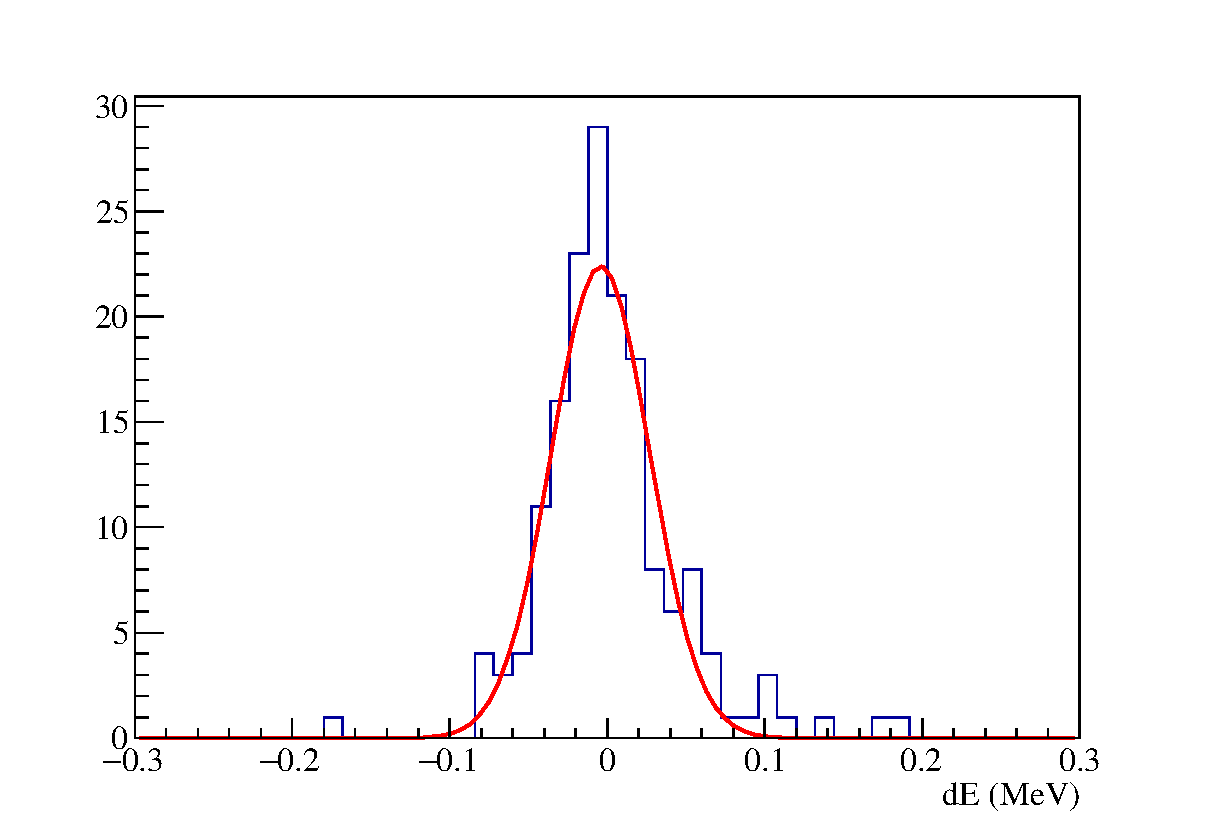
\includegraphics[clip, width=\columnwidth]{dE_10020_mod.eps}
    \caption{\Methane の場合の$dE$.}
    \label{fig::dE_ch4}
  \end{minipage}
\end{figure}
\begin{figure}
  \begin{minipage}{0.45\columnwidth}
    \centering
    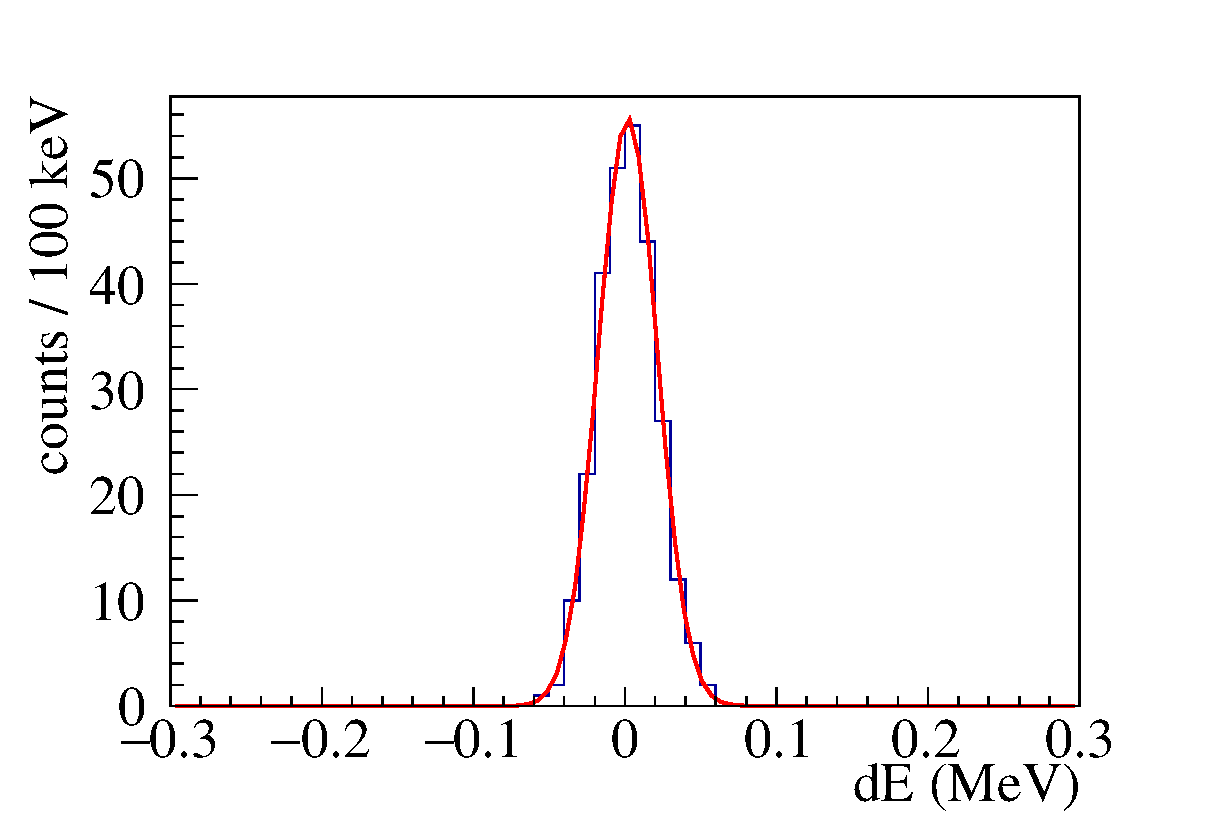
\includegraphics[clip, width=\columnwidth]{dE_10022_mod.eps}
    \caption{\MethaneHydro の場合の$dE$.}
    \label{fig::dE_ch4_h2}
  \end{minipage}
  \centering
  \begin{minipage}{0.45\columnwidth}
    \centering
    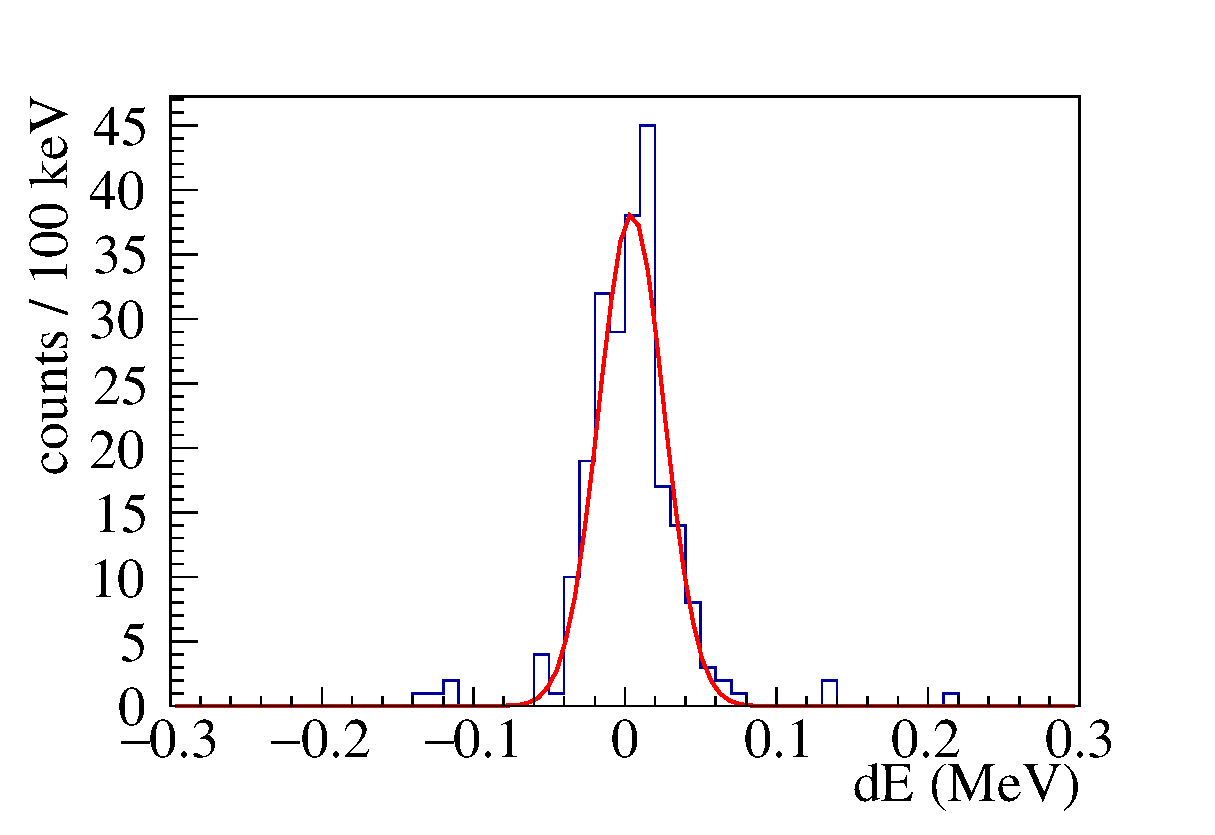
\includegraphics[clip, width=\columnwidth]{dE_10021_mod.eps}
    \caption{\MethaneHerium の場合の$dE$.}
    \label{fig::dE_ch4_he}
  \end{minipage}
\end{figure}
\begin{figure}
  \begin{minipage}{0.45\columnwidth}
    \centering
    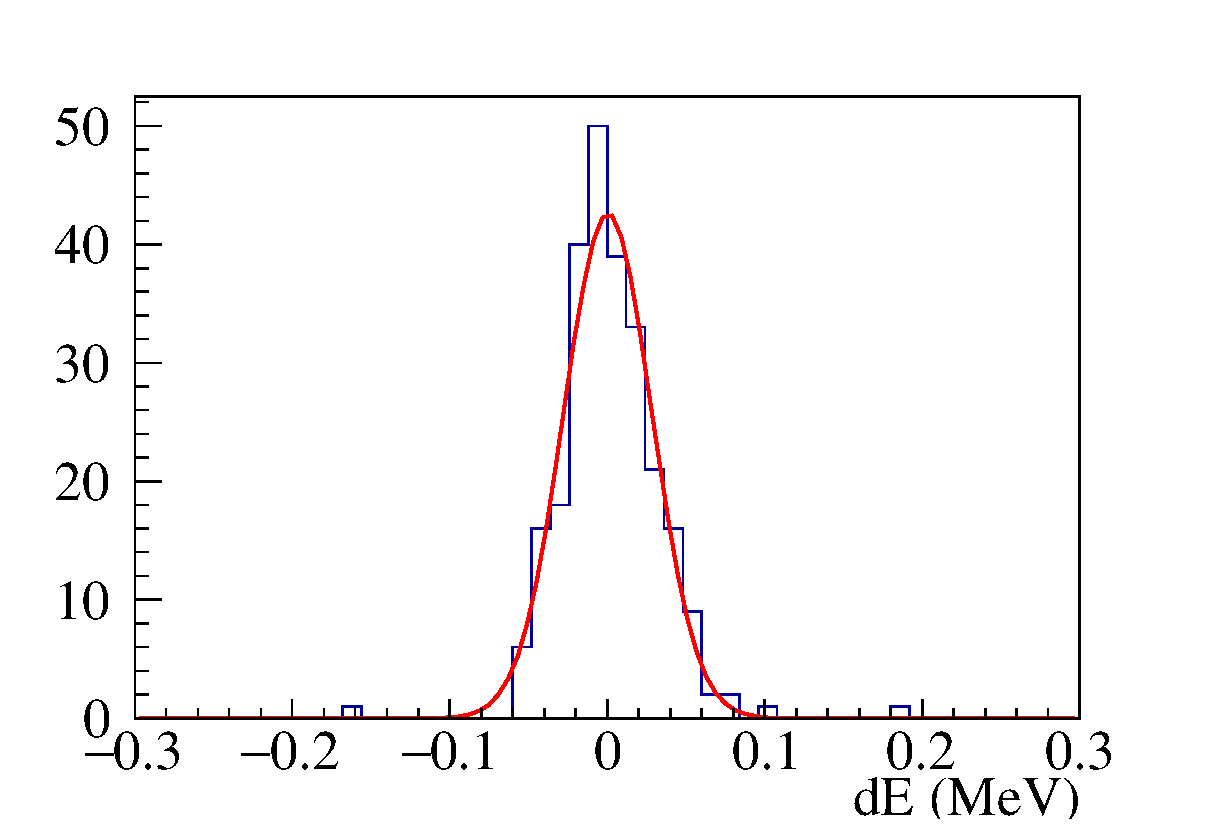
\includegraphics[clip, width=\columnwidth]{dE_10024_mod.eps}
    \caption{\isoButaneHydro の場合の$dE$.}
    \label{fig::dE_ic4h10_h2}
  \end{minipage}
  \centering
  \begin{minipage}{0.45\columnwidth}
    \centering
    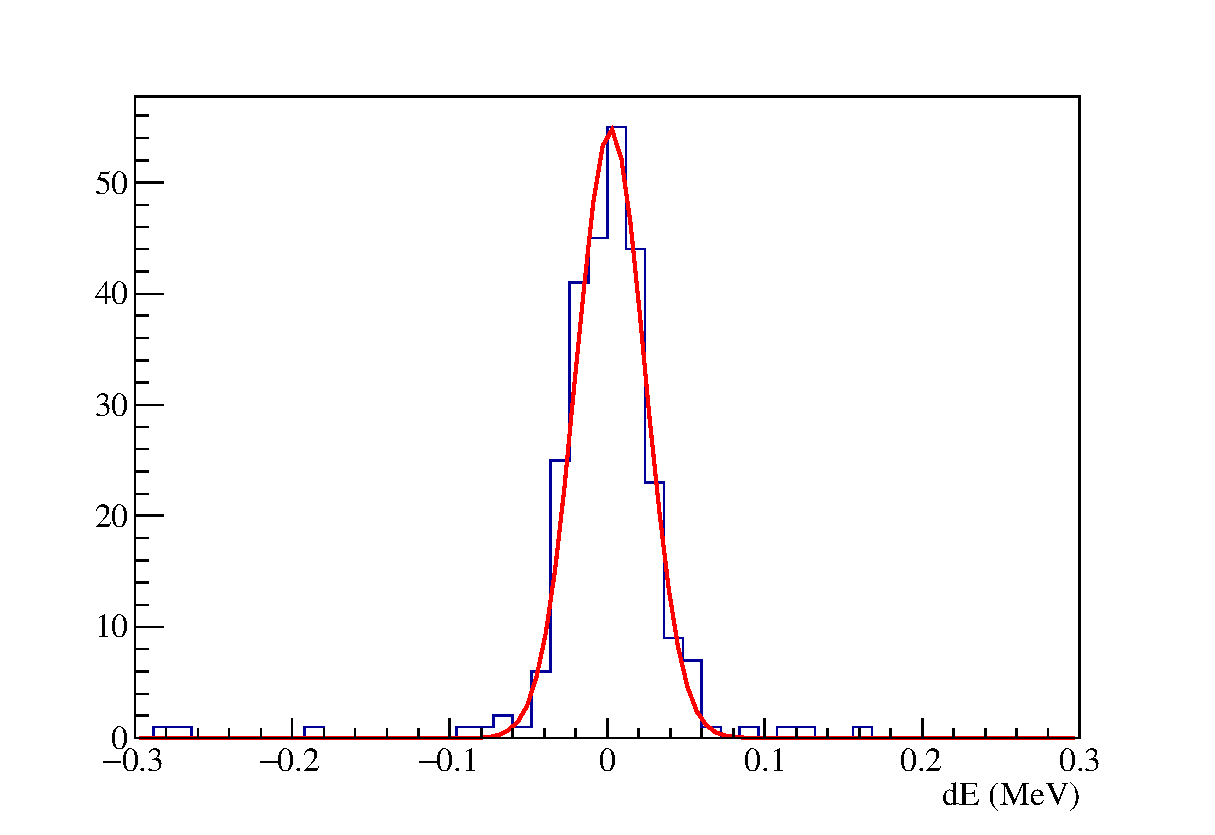
\includegraphics[clip, width=\columnwidth]{dE_10023_mod.eps}
    \caption{\isoButaneHerium の場合の$dE$.}
    \label{fig::dE_ic4h10_he}
  \end{minipage}
\end{figure}
%\begin{table}
%  \centering
%  \caption{エネルギーの差分.}
%  \label{tab::energy_resolution}
%  \begin{tabular}{ccc}
%    \toprule
%    gas & $dE$ (keV) & $\sigma$ (keV) \\
%    \midrule
%    \Methane  & 11.0 & 33.0  \\
%    \MethaneHydro & 1.25 & 20.0 \\
%    \MethaneHerium  & 9.30 & 23.7 \\
%    \isoButaneHydro  & 4.56 & 23.6 \\
%    \isoButaneHerium  & 5.00 & 22.3 \\
%    \bottomrule
%  \end{tabular}
%\end{table}
エネルギー分解能は,他と比較して\MethaneHydro の場合に最も小さいことが分かる.
%混合ガスの場合,分散は約20 keV となっている.

\subsection{角度分解能}
シミュレーションでの$\alpha$粒子の角度とeye-scanでの角度の差分を$d\theta$とする.
各ガスでの$d\theta$の分布を図\ref{fig::dtheta_ch4}, \ref{fig::dtheta_ch4_h2}, \ref{fig::dtheta_ch4_he},
\ref{fig::dtheta_ic4h10_h2}, \ref{fig::dtheta_ic4h10_he}に,
分布の中心値と分散を表\ref{tab::gas_summary}に示す.
\begin{figure}
  \centering
  \begin{minipage}{0.45\columnwidth}
    \centering
    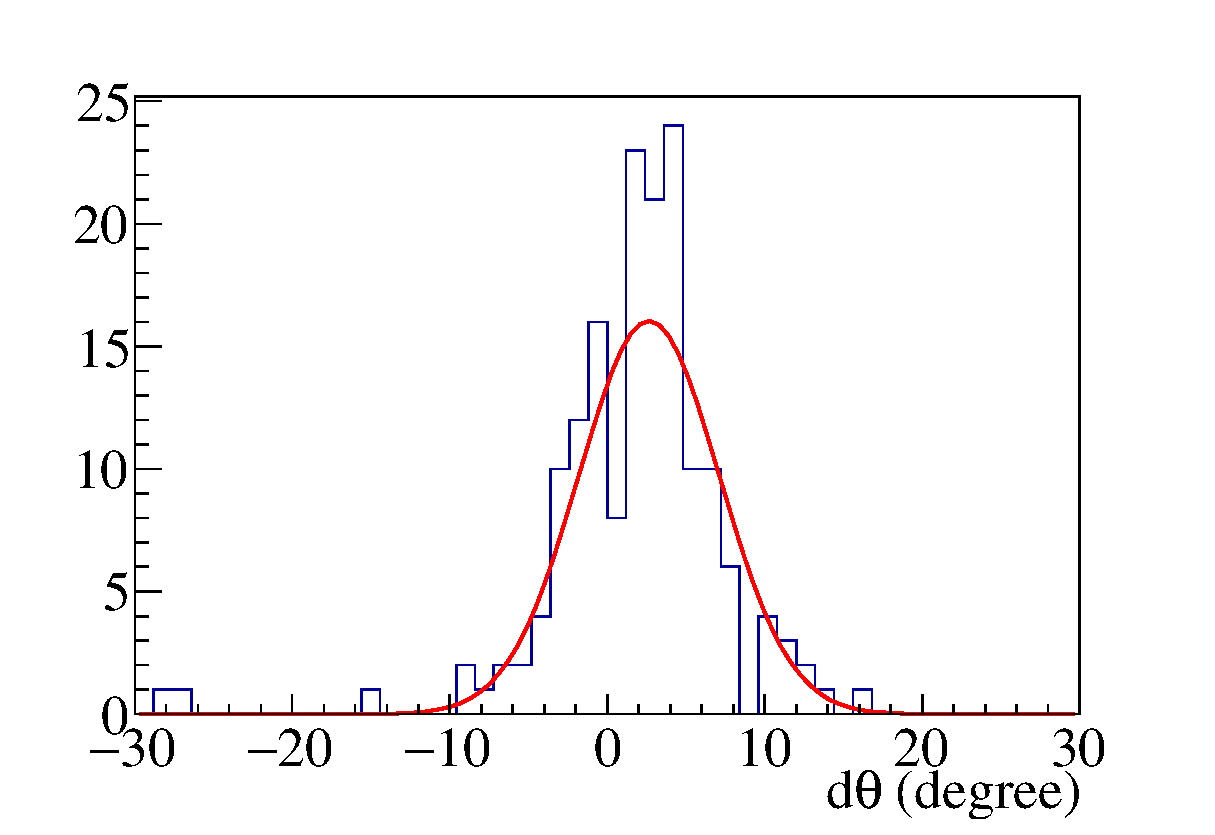
\includegraphics[clip, width=\columnwidth]{dtheta_10020_fit.eps}
    \caption{\Methane の場合の角度差.}
    \label{fig::dtheta_ch4}
  \end{minipage}  
\end{figure}
\begin{figure}
  \centering
  \begin{minipage}{0.45\columnwidth}
    \centering
    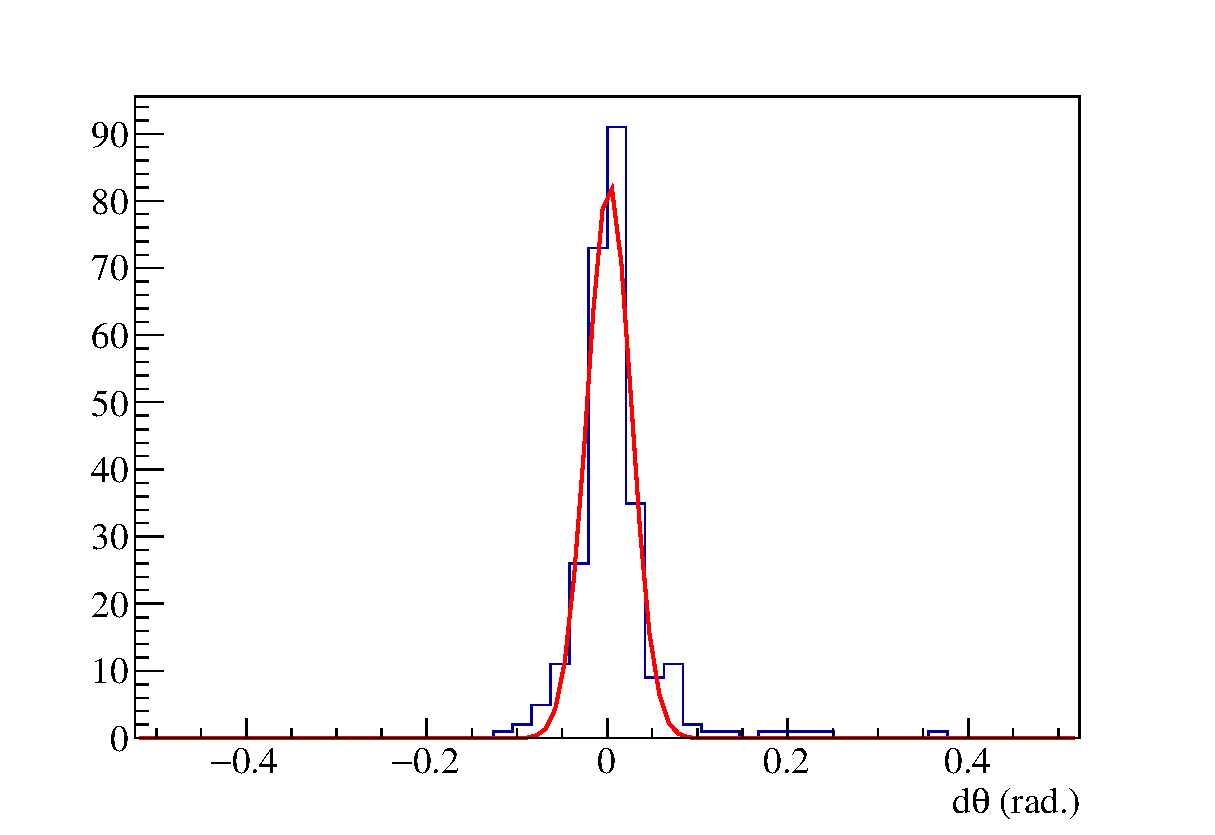
\includegraphics[clip, width=\columnwidth]{dtheta_10022_fit.eps}
    \caption{\MethaneHydro の場合の角度差.}
    \label{fig::dtheta_ch4_h2}
  \end{minipage}
  \begin{minipage}{0.45\columnwidth}
    \centering
    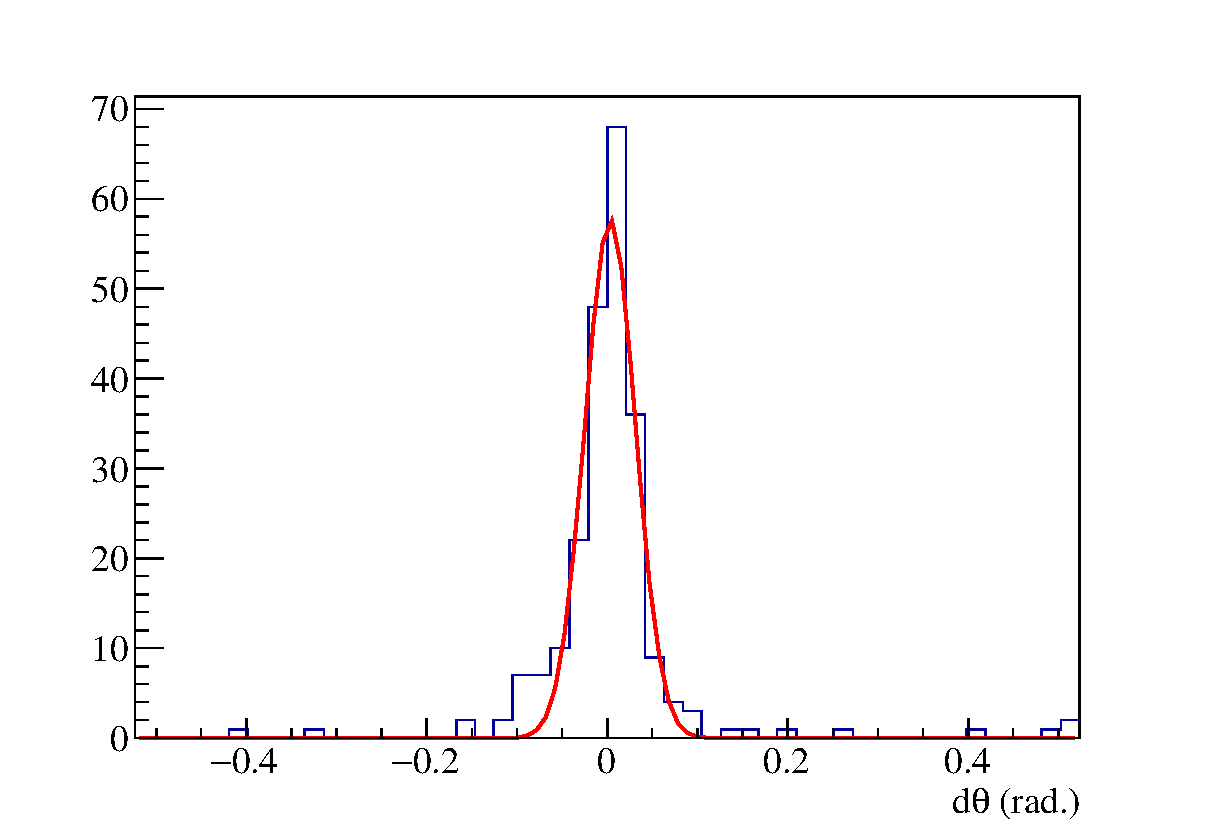
\includegraphics[clip, width=\columnwidth]{dtheta_10021_fit.eps}
    \caption{\MethaneHerium の場合の角度差.}
    \label{fig::dtheta_ch4_he}
  \end{minipage}
\end{figure}
\begin{figure}
  \centering
  \begin{minipage}{0.45\columnwidth}
    \centering
    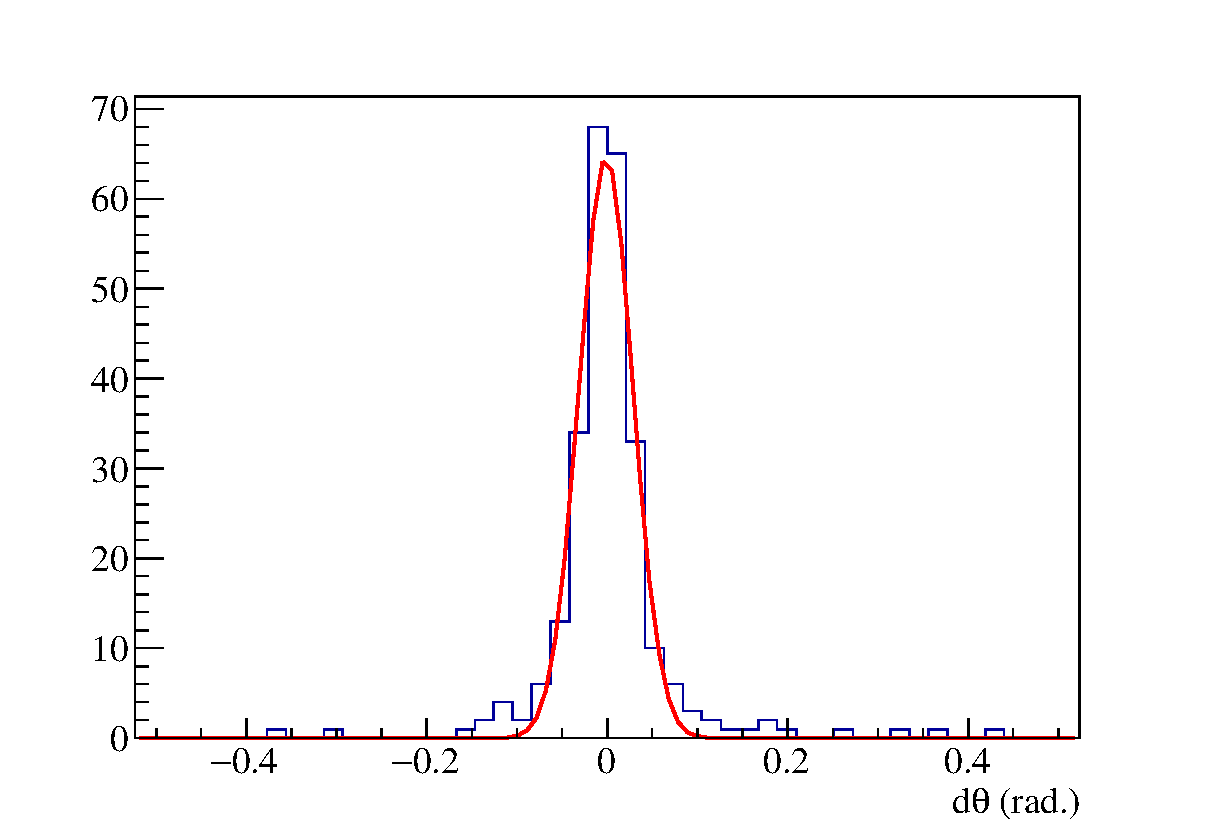
\includegraphics[clip, width=\columnwidth]{dtheta_10024_fit.eps}
    \caption{\isoButaneHydro の場合の角度差.}
    \label{fig::dtheta_ic4h10_h2}
  \end{minipage}
  \begin{minipage}{0.45\columnwidth}
    \centering
    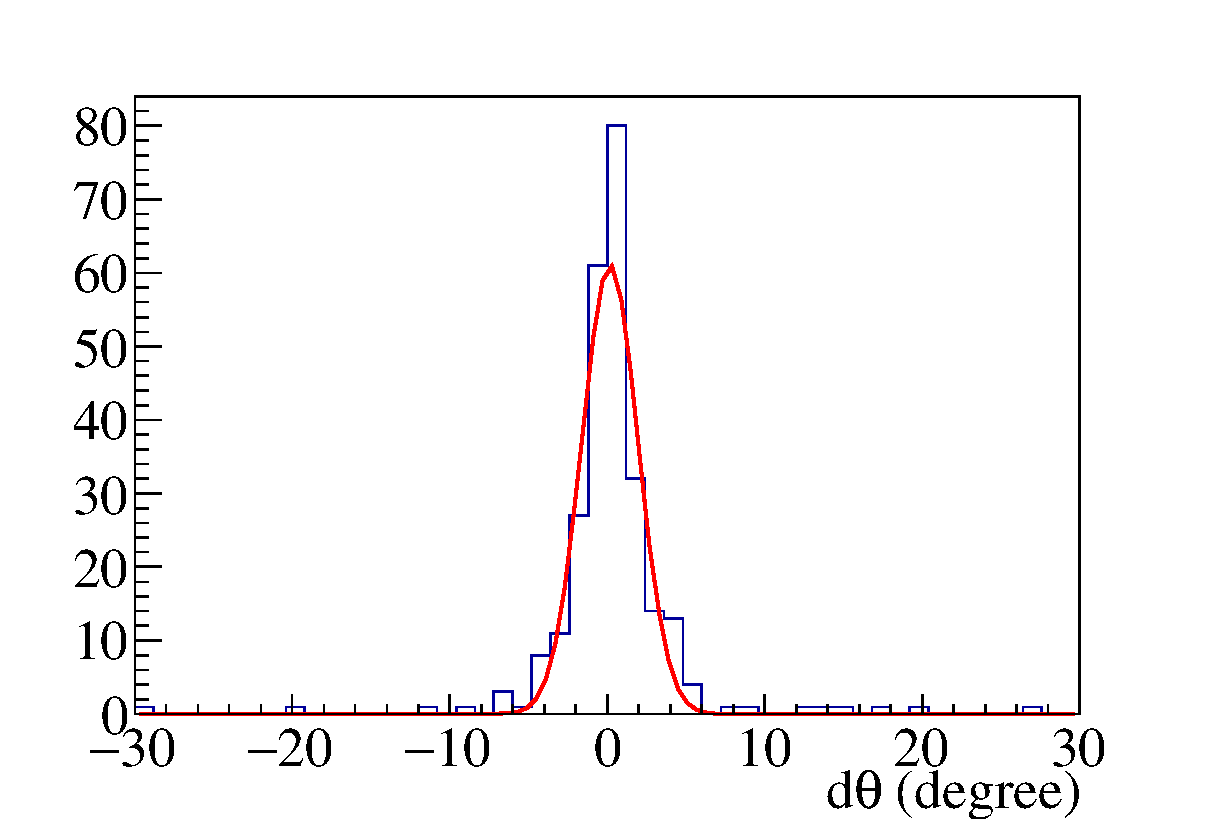
\includegraphics[clip, width=\columnwidth]{dtheta_10023_fit.eps}
    \caption{\isoButaneHerium の場合の角度差.}
    \label{fig::dtheta_ic4h10_he}
  \end{minipage}
\end{figure}
%\begin{table}
%  \centering
%  \caption{角度の差分.}
%  \label{tab::theta_resolution}
%  \begin{tabular}{ccc}
%    \toprule
%    gas & $d\theta$ (mrad.) & $\sigma$ (mrad.) \\
%    \midrule
%    \Methane  & 46.4 & 77.9 \\
%    \MethaneHydro & 2.10 & 24.6 \\
%    \MethaneHerium  & 3.34 & 28.2 \\
%    \isoButaneHydro  & -1.27 & 29.8 \\
%    iso-$\mathrm{C}_{4}\mathrm{H}_{10}\ (1) + \mathrm{He}\ (9) $ & 3.05 & 31.4 \\
%    \midrule
%  \end{tabular}
%\end{table}
角度分解能は,他と比較して\Methane 単体の場合に大きいことが分かる.

\subsection{励起エネルギー分解能}
測定で${}^{12}\mathrm{C}$の励起状態を特定する際に,
励起エネルギーの分解能が悪ければ各状態を分離することができない.
シミュレーションではHoyle状態経由での崩壊を考えているので,
${}^{12}\mathrm{C}$の励起エネルギーは7.65 MeV となっている.
eye-scanで決定した不変質量から基底状態の${}^{12}\mathrm{C}$の質量を引くことで励起エネルギーを求め,
7.65 MeV を再構築できるか評価する.
各ガスで再構成した励起エネルギーを図\ref{fig::Ex_ch4}, \ref{fig::Ex_ch4_h2}, \ref{fig::Ex_ch4_he},
\ref{fig::Ex_ic4h10_h2}, \ref{fig::Ex_ic4h10_he}, 表\ref{tab::gas_summary}に示す.
\begin{figure}
  \centering
  \begin{minipage}{0.45\columnwidth}
    \centering
    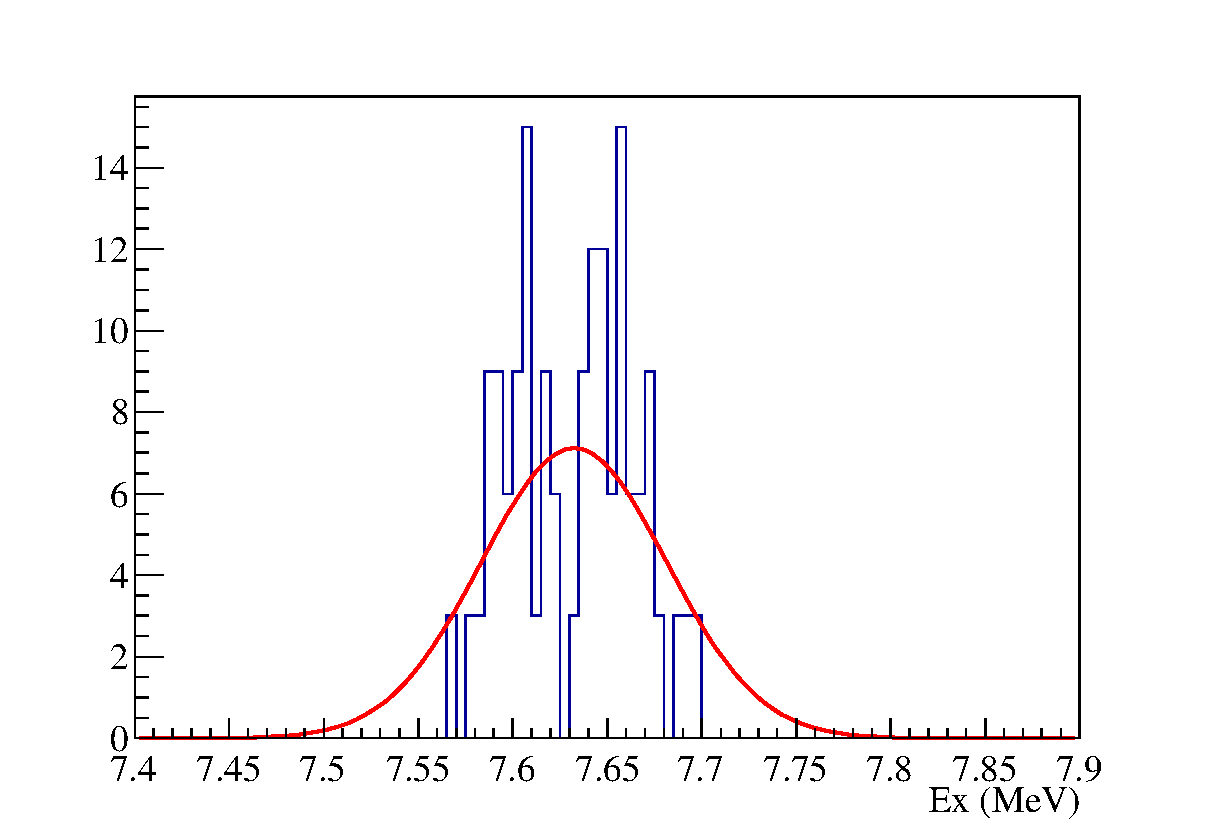
\includegraphics[clip, width=\columnwidth]{Ex_10020_fit.eps}
    \caption{\Methane の場合の${}^{12}\mathrm{C}$の励起エネルギー.}
    \label{fig::Ex_ch4}
  \end{minipage}
\end{figure}
\begin{figure}
  \centering
  \begin{minipage}{0.45\columnwidth}
    \centering
    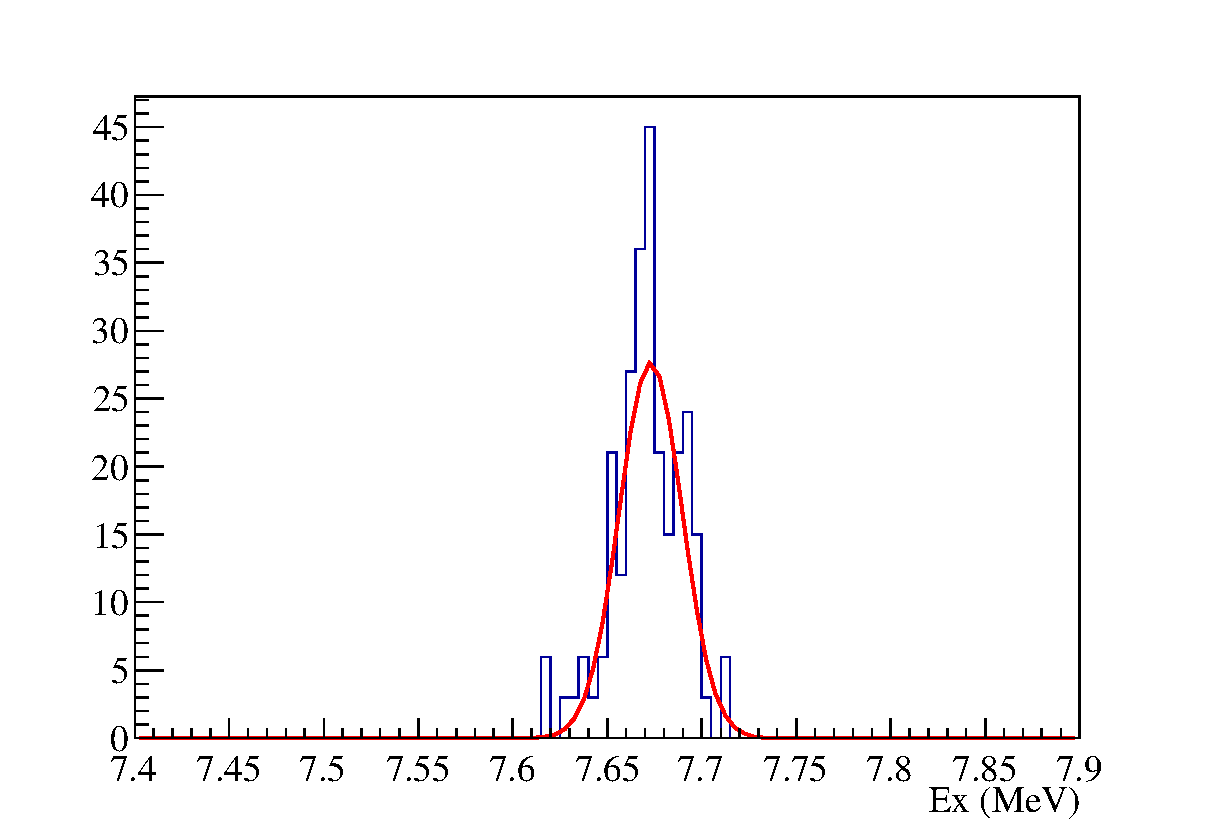
\includegraphics[clip, width=\columnwidth]{Ex_10022_fit.eps}
    \caption{\MethaneHydro の場合の${}^{12}\mathrm{C}$の励起エネルギー.}
    \label{fig::Ex_ch4_h2}
  \end{minipage}
  \begin{minipage}{0.45\columnwidth}
    \centering
    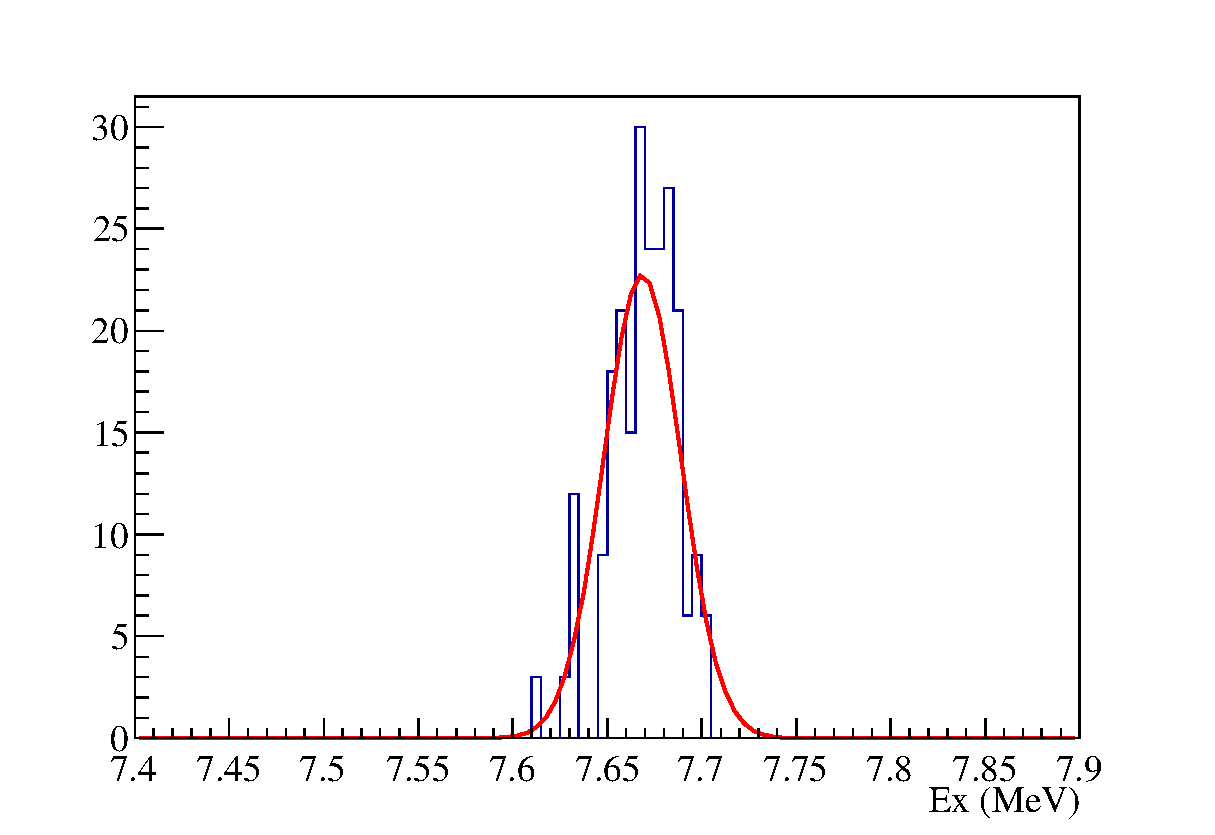
\includegraphics[clip, width=\columnwidth]{Ex_10021_fit.eps}
    \caption{\MethaneHerium の場合の${}^{12}\mathrm{C}$の励起エネルギー.}
    \label{fig::Ex_ch4_he}
  \end{minipage}
\end{figure}
\begin{figure}
  \centering
  \begin{minipage}{0.45\columnwidth}
    \centering
    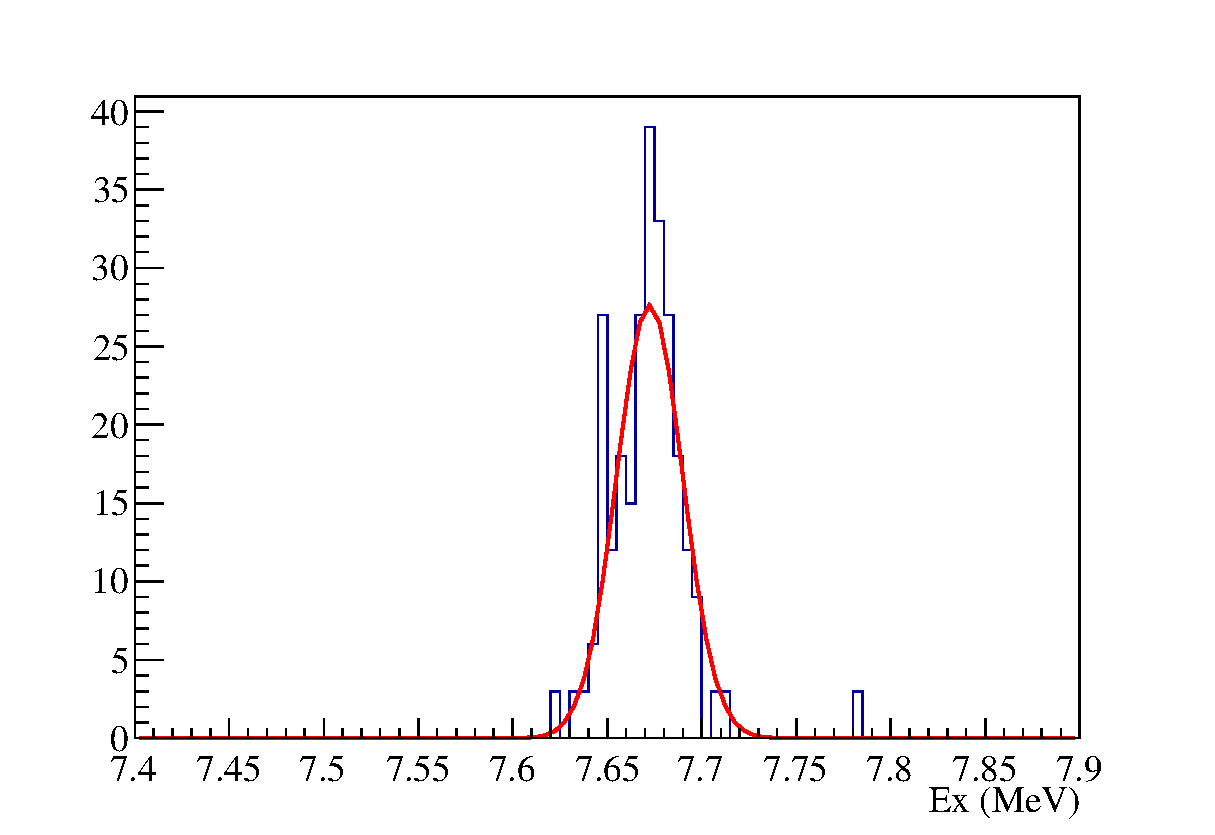
\includegraphics[clip, width=\columnwidth]{Ex_10024_fit.eps}
    \caption{\isoButaneHydro の場合の${}^{12}\mathrm{C}$の励起エネルギー.}
    \label{fig::Ex_ic4h10_h2}
  \end{minipage}
  \begin{minipage}{0.45\columnwidth}
    \centering
    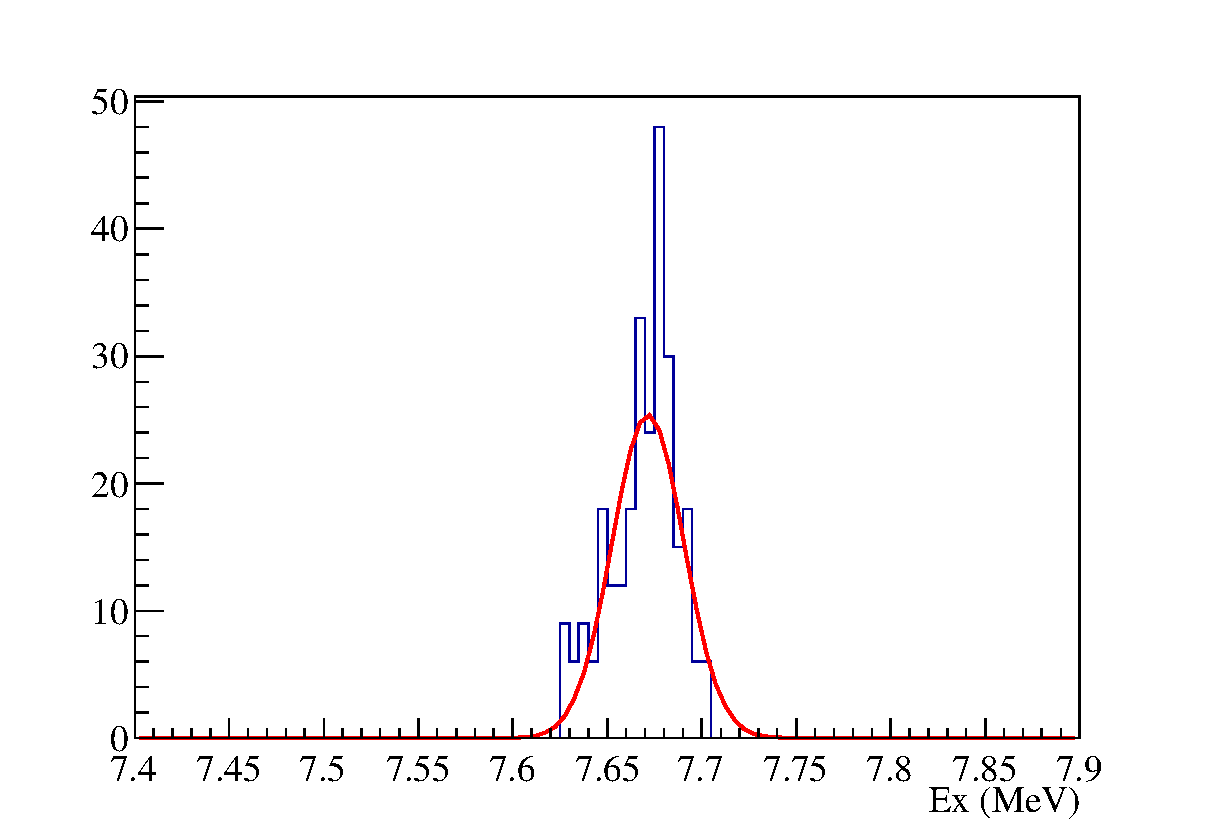
\includegraphics[clip, width=\columnwidth]{Ex_10023_fit.eps}
    \caption{\isoButaneHerium の場合の${}^{12}\mathrm{C}$の励起エネルギー.}
    \label{fig::Ex_ic4h10_he}
  \end{minipage}
\end{figure}
%\begin{table}
%  \centering
%  \caption{各ガスで求めた励起エネルギー.}
%  \label{tab::Ex_resolution}
%  \begin{tabular}{ccc}
%    \toprule
%    gas & Ex (MeV) & $\sigma$ (MeV) \\
%    \midrule
%    \Methane  & 7.63 & $4.91\times 10^{-2}$ \\
%    \MethaneHydro & 7.67 & $1.66\times 10^{-2}$ \\
%    \MethaneHerium  & 7.67 & $2.05\times 10^{-2}$ \\
%    \isoButaneHydro  & 7.67 & $1.75\times 10^{-2}$ \\
%    \isoButaneHerium  & 7.67 & $1.90\times 10^{-2}$ \\
%    \bottomrule
%  \end{tabular}
%\end{table}
Hoyle状態を再構成できていることが分かる.
また,分解能も他の状態と分けるのに十分良いことも分かる.

\begin{table}
  \caption{各ガスの検出効率と分解能.それぞれ100 eventsずつeye-scanによって解析を行った.}
  \label{tab::gas_summary}
  \begin{tabular}{ccccc}
    \toprule
    gas & 検出効率 (\%) & 
    $dE\pm\sigma$ (\si{\kilo\electronvolt}) &
    $d\theta\pm\sigma$ (\si{\milli\radian}) &
    Ex$\pm\sigma$ (\si{\mega\electronvolt})\\
    \midrule
    \Methane  & 55 & $-4.21\times10^{-3}\pm3.13\times10^{-2}$ & $46.4\pm77.9$ & $7.63\pm4.91\times10^{-2}$ \\
    \MethaneHydro & 91 & $1.36\times10^{-3}\pm1.97\times10^{-2}$ & $2.10\pm24.6$ & $7.67\pm1.66\times10^{-2}$ \\
    \MethaneHerium & 78 & $3.75\times10^{-3}\pm2.34\times10^{-2}$ & $3.34\pm28.2$ & $7.67\pm2.05\times10^{-2}$ \\
    \isoButaneHydro  & 87 & $3.75\times10^{-4}\pm2.80\times10^{-2}$ & $-1.27\pm29.8$ & $7.67\pm1.75\times10^{-2}$ \\
    \isoButaneHerium  & 90 & $2.14\times10^{-3}\pm2.20\times10^{-2}$ & $3.05\pm31.4$ & $7.67\pm1.90\times10^{-2}$ \\
    \bottomrule
  \end{tabular}
\end{table}

\section{検出ガスの決定}
ディフュージョンとトラックの幅の観点では\MethaneHydro ,
\isoButaneHydro  が良い.
検出効率は\MethaneHydro , \isoButaneHydro ,
\isoButaneHerium が良い.
$\alpha$粒子のエネルギー分解能の観点では\MethaneHydro が良い.
角度分解能の観点では\MethaneHydro ,
\isoButaneHydro が良い.
これらから考えると,\MethaneHydro または
\isoButaneHydro が適すると判断できる.
\MethaneHydro と \isoButaneHydro とで
含まれる${}^{12}\mathrm{C}$の量を比較すると,
\isoButaneHydro の方が4/3倍多い.
よって,検出ガスには\isoButaneHydro を用いる.

\end{document}
